%\documentclass[12pt,handout]{beamer}
%\documentclass{beamer}
\usepackage[ngerman]{babel}
\usepackage[ansinew]{inputenc}
\usepackage{amsmath}
\usepackage{amssymb}
\usepackage{listings} 
\usepackage{stmaryrd}
\lstset{language=Python, tabsize=4, showstringspaces=false,basicstyle=\footnotesize,mathescape=true}  
\usepackage{mathtools}
\usepackage{ulem}
\usepackage{tikz}

\usetheme{Boadilla}
\mode<presentation>{
\useoutertheme[subsection=false]{miniframes}
\useinnertheme{rectangles}
%\usecolortheme{crane}
}
\parskip 10pt



\begin{document}
\title{Informatik}   
\author{Graphen 2} 
\date{}
\frame{\titlepage} 

%---

\begin{frame}[fragile]

\begin{minipage}[c]{5cm}
Erreichbarkeit

Gegeben ein Graph G und ein Startknoten s. Welche Knoten sind von s erreichbar?
\end{minipage}
\begin{minipage}[c]{6cm}
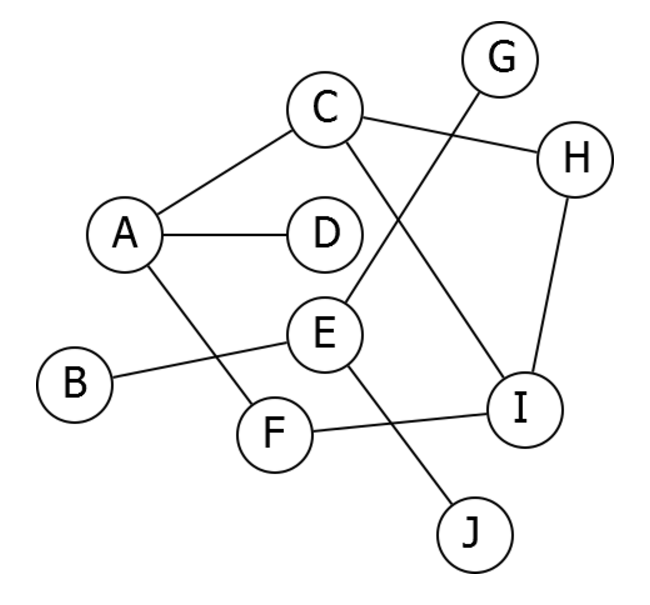
\includegraphics[width=5cm]{bild2.png}
\end{minipage}   \pause

\begin{lstlisting}
Setze alle Knoten auf nicht besucht
explore(s)
Gib alle Knoten aus, die besucht wurden

def explore(v): 
    merke v als besucht
    f�r alle Nachbarn w von v:
        wenn w nicht besucht:
            explore(w)

\end{lstlisting}

\end{frame}

\begin{frame}[fragile]

\begin{lstlisting}
visited =  {v : False for v in G}       
def explore(v):  
    visited[v] = True
    for w in G[v]:
        if not visited[w]:
            explore(w) 
 
explore(s)
result = [v for v in G if visited[v]]            
print(*result)
\end{lstlisting}   $\pause$
Die Funktion explore realisiert eine rekursive Tiefensuche (dfs, depth first search).

Laufzeit:  $\pause$ jeder Knoten wird h�chstens einmal explored:  $O(\left|V\right|)$, jeder Knoten pr�ft seine Nachbarn, 
die Zahl der Nachbarn liegt in  $O(\left|E\right|)$, insgesamt also   $O(\left|V\right|+\left|E\right|)$.
\end{frame}

\begin{frame}[fragile]
Es gilt: Die Knoten eines ungerichteten Graphen G k�nnen in \textbf{Zusammenhangskomponenten} (Connected Components) aufgeteilt werden, so dass v von w genau dann erreichbar ist, wenn beide in derselben Zusammenhangskomponente liegen.

Bestimmung der Zusammenhangskomponenten:  

\begin{lstlisting} [basicstyle=\tiny]
Setze alle Knoten auf nicht besucht
Setze die Komponentennummer aller Knoten auf 0
cc = 1  # aktuelle Komponentennummer

F�r alle Knoten u in G:
    falls u noch nicht besucht:
        explore(u)
        cc += 1
Gib Resultat aus 

def explore(v):
    merke v als besucht
    merke cc als Komponentennummer von v
    f�r alle Nachbarn w von v:
        wenn w nicht besucht:
            explore(w)

\end{lstlisting} 

\end{frame}

\begin{frame}[fragile]

\begin{lstlisting} [basicstyle=\scriptsize]
visited = {v : False for v in G}  
ccnum = {v : 0 for v in G}     # Komponentennummer von v
cc = 1                         # aktuelle Komponentennummer    

def explore(v):
    visited[v] = True
    ccnum[v] = cc
    for w in G[v]:
        if not visited[w]:
            explore(w)   

for v in G.keys():
    if not visited[v] :
        explore(v)
        cc+=1 
      
for i in range(1,cc):
    result = [v for v in G if ccnum[v] $==$ i]   
    print(i,'-',*result)
\end{lstlisting} 

Laufzeit: $\pause O(\left|V\right|+\left|E\right|)$.
\end{frame}

\begin{frame}[fragile]
DFS endet damit, dass alle Knoten markiert sind. Das ist
als Ergebnis noch nicht sonderlich interessant. Interessant wird 
DFS daduch, dass man bei der Ausf�hrung noch Daten sammelt, z.B. die previsit und postvisit Nummern.

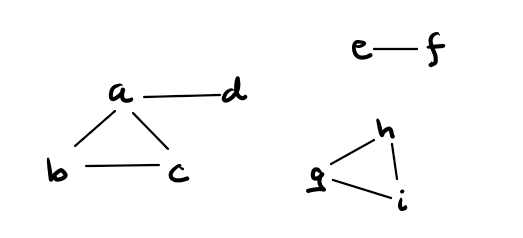
\includegraphics[width=9cm]{bild7.png}

\end{frame}

\begin{frame}[fragile]

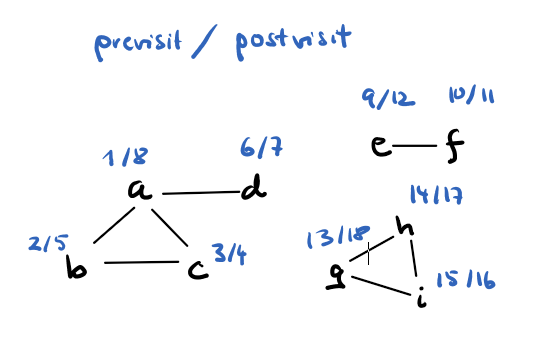
\includegraphics[width=8cm]{bild8.png}   $\pause$         

F�r alle Knoten u und v gilt: die Intervalle [pre(u),post(u)] und [pre(v),post(v)] sind entweder
ineinander verschachtelt oder disjunkt.
\end{frame}

\begin{frame}[fragile]
Bestimmung der previsit und postvisit-Nummern der Tiefensuche
\begin{lstlisting} 
Setze alle Knoten auf nicht besucht
Setze previsit und postvisit Nummer aller Knoten auf 0
counter = 1  # Z�hler f�r die visit-Nummer

F�r alle Knoten u in G:
    falls u noch nicht besucht:
        explore(u)
Gib Resultat aus

def explore(v):
    merke v als besucht
    setze previsit-Nummer von v auf counter
    erh�he counter um 1
    f�r alle Nachbarn w von v:
        wenn w nicht besucht:
            explore(w)
    setze postvisit-Nummer von v auf counter
    erh�he counter um 1

\end{lstlisting} 
\end{frame}

\begin{frame}[fragile] 
\begin{lstlisting} [basicstyle=\scriptsize]
visited = {v : False for v in G}  
previsit = {v : 0 for v in G}         
postvisit = {v : 0 for v in G}     
counter = 1

def explore(v):
    global counter
    visited[v] = True
    previsit[v] = counter
    counter += 1
    for w in G[v]:
        if not visited[w]:
            explore(w)
    postvisit[v] = counter
    counter += 1

for v in G.keys():
    if not visited[v] :
        explore(v)

for v in G:
    print("{:2} {:1} {:2}".format(previsit[v],v,postvisit[v]))
\end{lstlisting} 
\end{frame}

\begin{frame}[fragile] 
Topologische Sortierung eines gerichteten Graphen: wir wollen eine Nummerierung der Knoten finden, die mit den Kantenrichtungen
kompatibel ist.

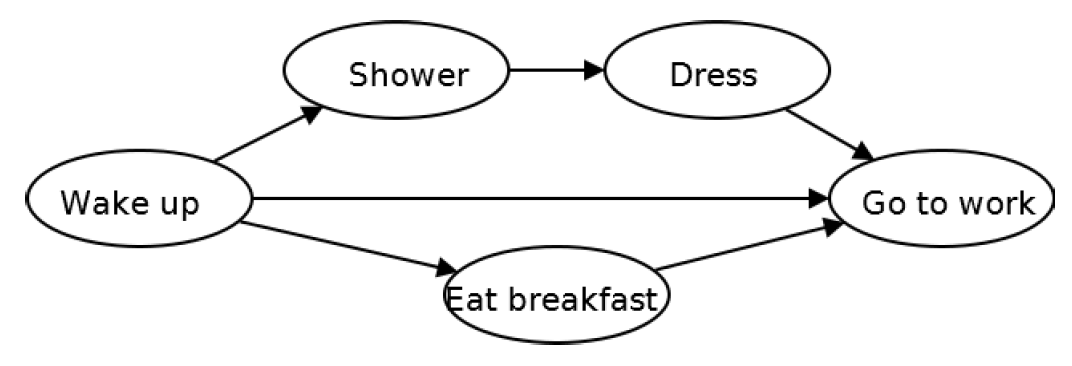
\includegraphics[width=7cm]{bild9.png} $\pause$         

Es gilt: ein Graph kann genau dann topologisch sortiert werden, wenn er keinen Kreis enth�lt.
Anders formuliert: Genau die gerichteten azyklischen Graphen (directed acyclic graph, DAG) k�nnen topologisch sortiert werden. 

\end{frame}

\begin{frame}[fragile] 
Eine Quelle (source) ist ein Knoten mit dem Eingangsgrad 0. Eine Senke (sink) ist ein Knoten mit dem Ausgangsgrad 0.

Bestimme die Senken des folgenden Graphen:

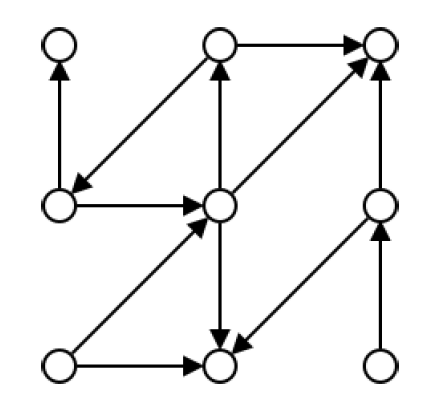
\includegraphics[width=6cm]{bild10.png}

\end{frame}

\begin{frame}[fragile] 

Idee f�r die topologische Sortierung (1. Versuch)
\begin{lstlisting} 
Solange der Graph nicht leer:
      Folge einem Pfad bis es nicht mehr weitergeht.
      Finde dort eine Senke
      F�ge die Senke in die Sortierung wie in einen Stapel ein
      Entferne die Senke aus dem Graphen.


\end{lstlisting} 
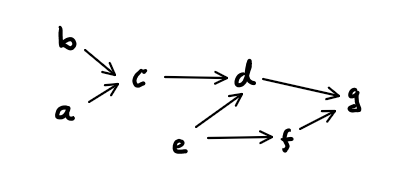
\includegraphics[width=6cm]{bild12.png}

Laufzeit:  $O(\left|V\right|^2)$    -   nicht gut

\end{frame}

\begin{frame}[fragile] 

Verbesserungsm�glichkeit: statt den Pfad immer wieder von vorne zu beginnen, wird nach der
Entfernung der Senke der Weg so weit wie n�tig zur�ckgegangen (backtrack).

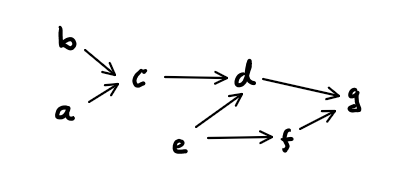
\includegraphics[width=6cm]{bild12.png}

Das ist Tiefensuche! Wir erhalten eine topologische Sortierung durch die postvisit-Nummerierung.



\end{frame}

\begin{frame}[fragile] 
\begin{lstlisting} 
visited = {v : False for v in G}  
postvisit = {v : 0 for v in G}     
counter = 1  

def explore(v):
    global counter
    visited[v] = True
    for w in G[v]:
        if not visited[w]:
            explore(w)
    postvisit[v] = counter
    counter += 1

for v in G:
    if not visited[v] :
        explore(v) 

result = sorted(G, key=lambda v: postvisit[v],reverse = True)
for i in range(len(result)):
    print(i+1,result[i])   
\end{lstlisting} 
\end{frame}

\begin{frame}[fragile] 
In einem gerichteten Graphen hei�en zwei Knoten u und v \textbf{zusammenh�ngend}, wenn u von v und v von u erreichbar ist.  $\pause$         

Es gilt: Ein gerichteter Graph kann partitioniert werden in \textbf{starke Zusammenhangskomponenten} (strongly connected components (SCC)), wobei zwei Knoten genau dann zusammenh�ngen, wenn sie in der selben Komponente sind.
\end{frame}

\begin{frame}[fragile] 
Finde die starken Zusammenhangskomponenten in dem Graphen.

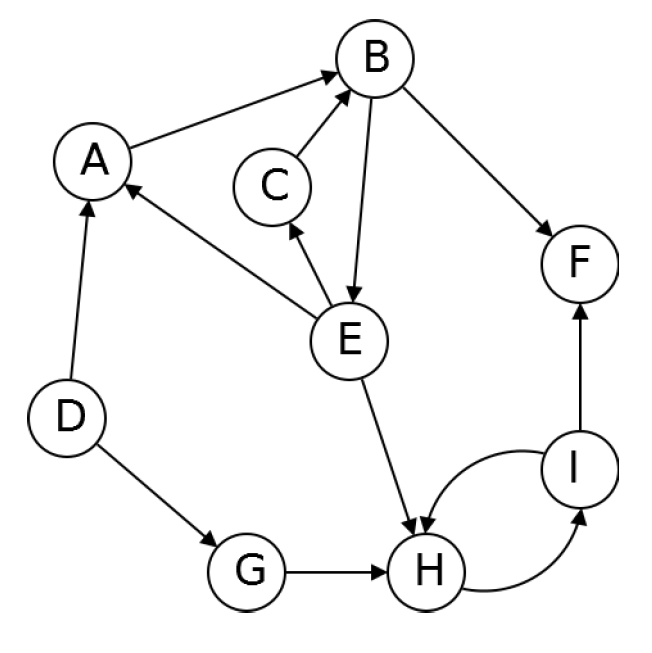
\includegraphics[width=6cm]{bild13.png}
\end{frame}

\begin{frame}[fragile] 

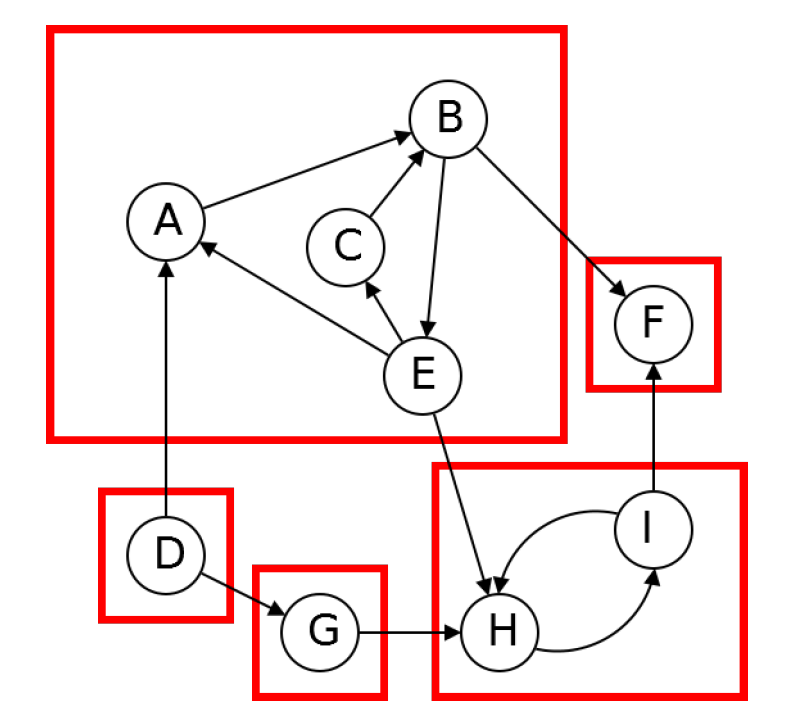
\includegraphics[width=7cm]{bild14.png}
\end{frame}

\begin{frame}[fragile] 
Der \textbf{Metagraph} zeigt, wie die starken Zusammenhangskomponenten untereinander verbunden sind.

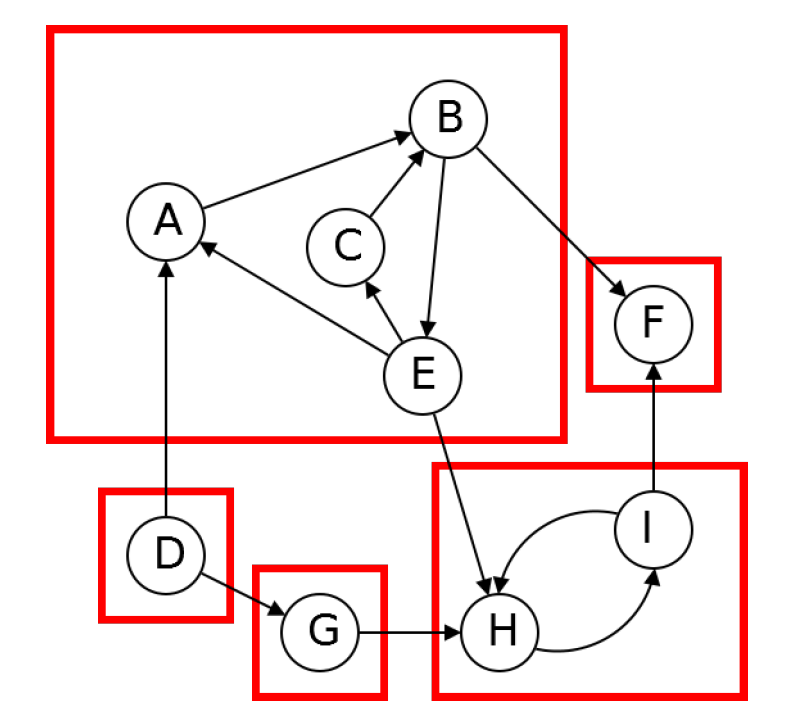
\includegraphics[width=5cm]{bild14.png}
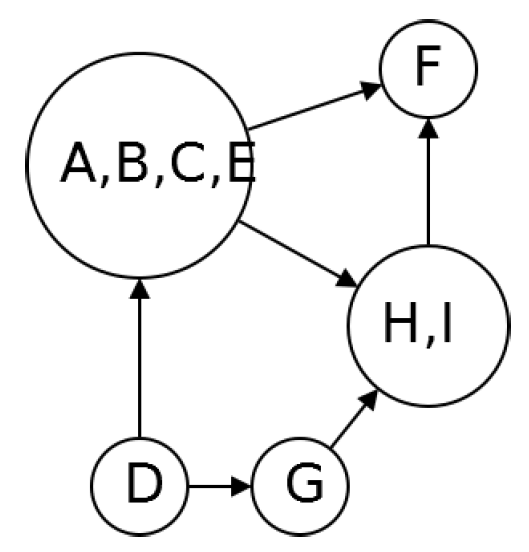
\includegraphics[width=4cm]{bild15.png}

Der Metagraph ist immer ein DAG.
\end{frame}

\begin{frame}[fragile] 
Wenn v in einer SCC-Senke liegt, dann findet explore(v) genau die Elemente des SCC.

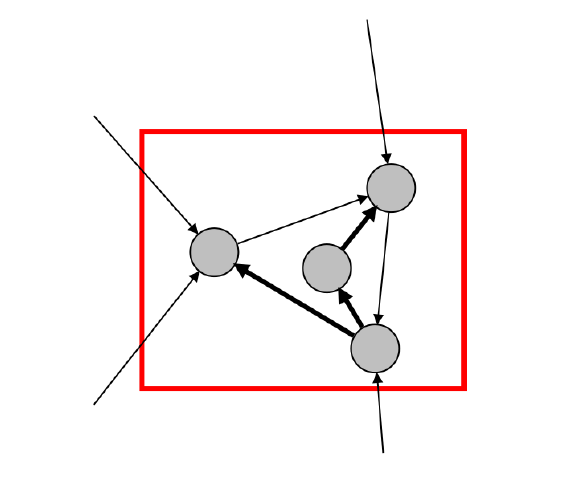
\includegraphics[width=6cm]{bild16.png}
\end{frame}

\begin{frame}[fragile] 
Es gilt: Wenn C und C' zwei starke Zusammenhangskomponenten sind und es eine Kante von einem Knoten aus C nach einem Knoten aus C' gibt, dann ist  die gr��te postvisit-Nummer in C gr��er als die gr��te postvisit-Nummer in C'. $\pause$    

Folgerung: der Knoten mit der gr��ten postvisit-Nummer ist in einer SCC-Quelle. Wir suchen aber eine SCC-Senke. $\pause$    

Dazu betrachten wir den transponierten Graphen. Den transponierten Graphen $G^T$ eines gerichteten Graphen G erh�lt man, wenn
man die Kantenrichtungen umdreht. $\pause$    

$G$ und $G^T$ haben dieselben SCCs. \\
SCC-Quellen in $G^T$ sind SCC-Senken in $G$.

\end{frame}

\begin{frame}[fragile]
Bestimmung der postvisit-Nummern des transponierten Graphen

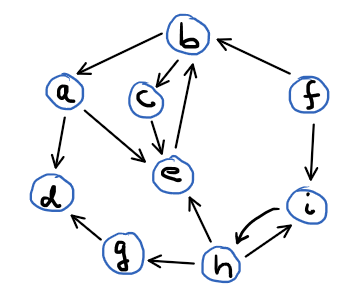
\includegraphics[width=5cm]{bild18.png} ~~  $\pause$    
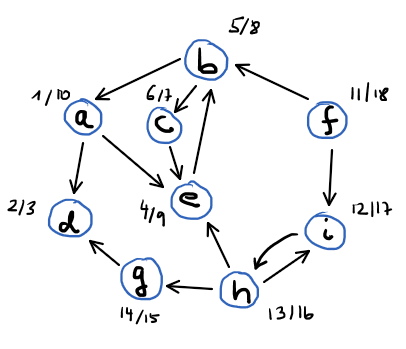
\includegraphics[width=5cm]{bild19.png}

\end{frame}

\begin{frame}[fragile]
�bertragung der postvisit-Nummern auf den Ausgangsgraphen

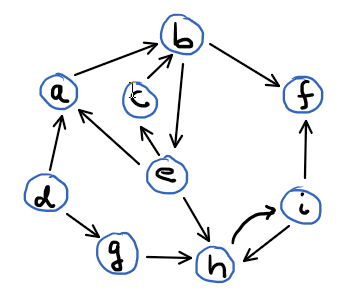
\includegraphics[width=6cm]{bild20.png} 
\end{frame}

\begin{frame}[fragile]
Bestimmung der SCCs mit Tiefensuche.

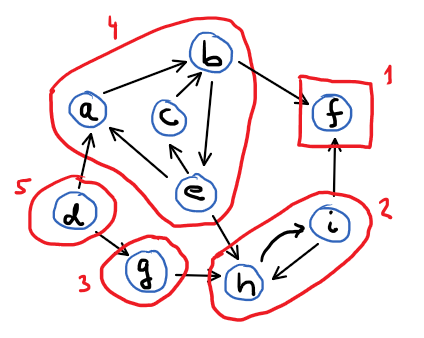
\includegraphics[width=6cm]{bild21.png} 

Laufzeit: im wesentlichen Tiefensuche auf $G^T$ und dann auf $G$, also  $O(\left|V\right|+\left|E\right|)$.
\end{frame}

\begin{frame}[fragile]
Bestimmung der starken Zusammenhangskomponenten in einem gerichteten Graphen $G$
\begin{lstlisting} 
F�hre Tiefensuche auf $G^T$ durch und merke postvisit-Nummern.
F�r alle Knoten v in G in umgekehrter postvisit-Nummerierung:
	Falls v noch nicht besucht:
		explore(v) und markiere alle
			 besuchten Knoten u als neuen SCC.
             

\end{lstlisting} 
\end{frame}

\begin{frame}[fragile]
\begin{minipage}[c]{4cm}
\begin{lstlisting}  [basicstyle=\tiny]
def exploreT(v):
    global counter
    visited[v] = True
    for w in Gt[v]:
        if not visited[w]:
            exploreT(w)
    postvisit[v] = counter
    counter+=1

def explore(v):
    visited[v] = True
    ccnum[v] = cc
    for w in G[v]:
        if not visited[w]:
            explore(w)
\end{lstlisting} 
\end{minipage} 
\begin{minipage}[c]{6cm}
\begin{lstlisting}  [basicstyle=\tiny]
Gt = {v:set() for v in G}
for v in G:
    for w in G[v]:
        Gt[w].add(v)
   
visited = {v : False for v in Gt}  
postvisit = {v : 0 for v in Gt}     
counter = 1       
for v in Gt:
    if not visited[v] :
        exploreT(v)    
        
vlist = sorted(Gt,key=lambda v: postvisit[v],reverse=True)
visited = {v : False for v in G}  
ccnum = {v : 0 for v in G}   
cc = 1

for v in vlist:
    if not visited[v] :
        explore(v)
        cc+=1

for i in range(1,cc):
    result = [v for v in G if visited[v] and ccnum[v] $==$ i]    
    print(i,'-',*result)
\end{lstlisting}
\end{minipage} 
\end{frame}
\end{document}